% ============================================================================
% FILE: sections/08_appendix.tex
% PURPOSE: รายละเอียดเพิ่มเติมที่ไม่ได้ใส่ในเนื้อหาหลัก
% ============================================================================

\appendix

% ============================================================
% Appendix A: รายละเอียด Engineering Drawing
% ============================================================

\section{รายละเอียด Engineering Drawing}
\label{app:drawings}

% ------------------------------------------------------------
\subsection{CAD Assembly (Full)}
\label{subsec:cad_assembly}
% ------------------------------------------------------------

\begin{figure}[H]
  \centering
  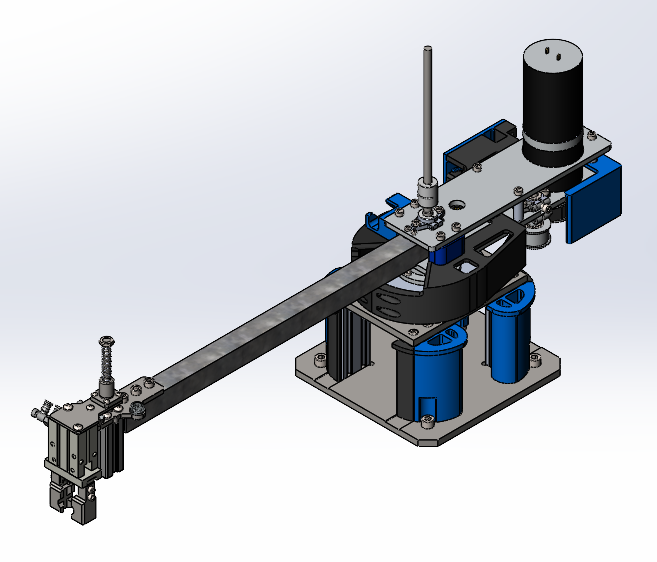
\includegraphics[width=0.95\textwidth]{images/Full_CAD.png}
  \caption{CAD Assembly ฉบับเต็ม แสดงทุกชิ้นส่วน}
  \label{fig:app_cad_full}
\end{figure}

% ------------------------------------------------------------
\subsection{Exploded View}
\label{subsec:exploded_view}
% ------------------------------------------------------------

\subsection*{A.2 Exploded View}

\textbf{1. ภาพรวม (Overview)}
\begin{figure}[H]
    \centering
    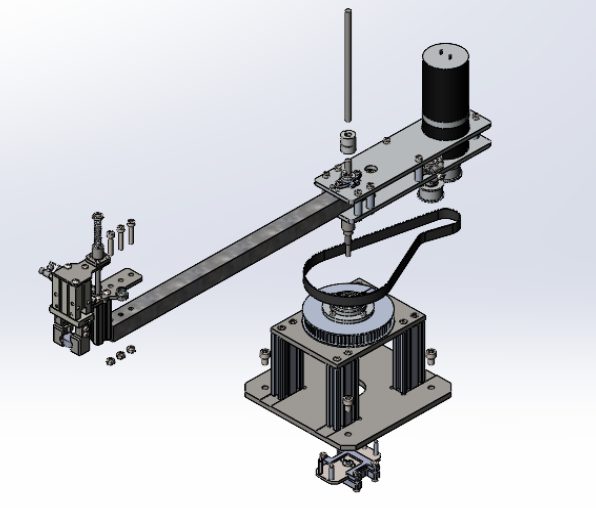
\includegraphics[width=0.8\textwidth]{images/assem_explode.png}
    \caption{รูป Exploded View ของหุ่นที่ไม่มี part จัดระเบียบสายไฟ ในมุม Isometric}
    \label{fig:overview_exploded_iso}
\end{figure}

\textbf{2. ส่วนฐาน (Base Sub-assembly)}
\begin{figure}[H]
    \centering
    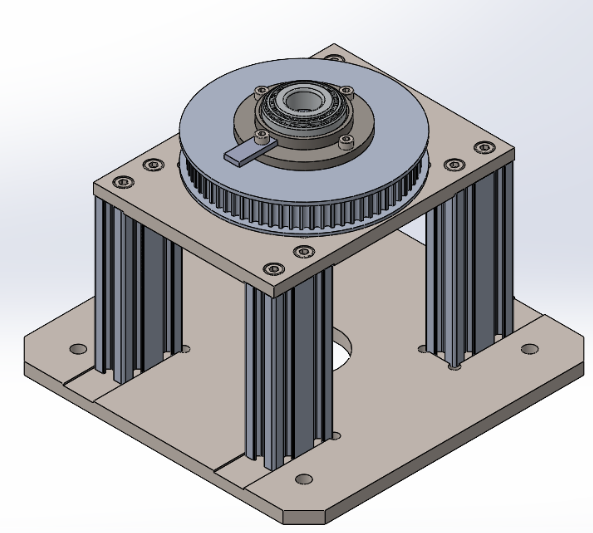
\includegraphics[width=0.7\textwidth]{images/Base_subassem.png}
    \caption{ภาพรวมของส่วนฐาน ในมุม Isometric}
    \label{fig:base_iso}
\end{figure}
\begin{figure}[H]
    \centering
    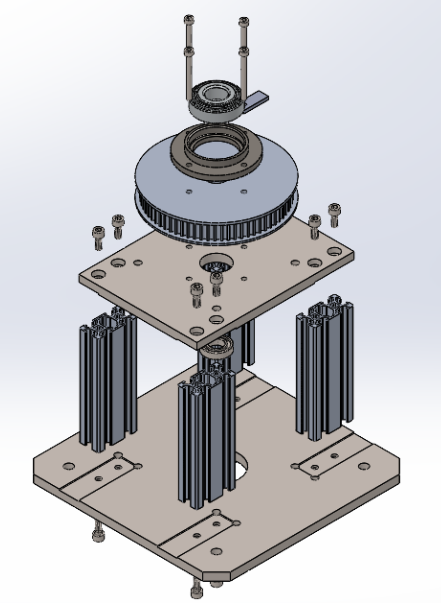
\includegraphics[width=0.8\textwidth]{images/Base_explode.png}
    \caption{รูป Exploded View ของส่วนฐานในมุม Isometric}
    \label{fig:base_exploded}
\end{figure}

\textbf{3. ส่วนแขนกลและข้อต่อ (Arm Links \& Joints)}
\begin{figure}[H]
    \centering
    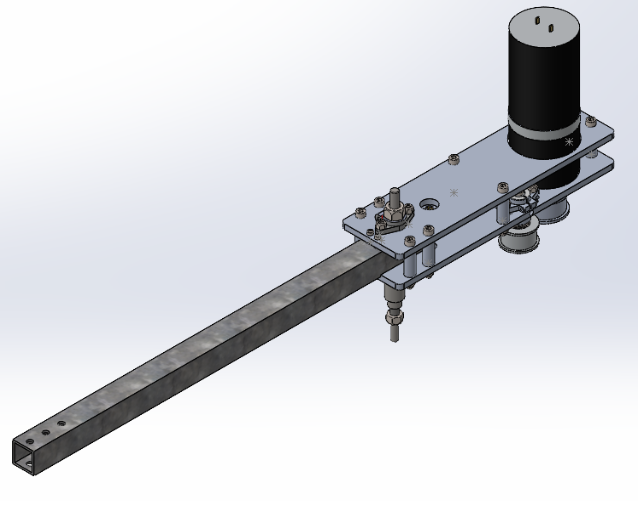
\includegraphics[width=0.7\textwidth]{images/Arm_subassem.png}
    \caption{ภาพรวมของส่วนแขนกลและข้อต่อ ในมุม Isometric}
    \label{fig:arm_iso}
\end{figure}
\begin{figure}[H]
    \centering
    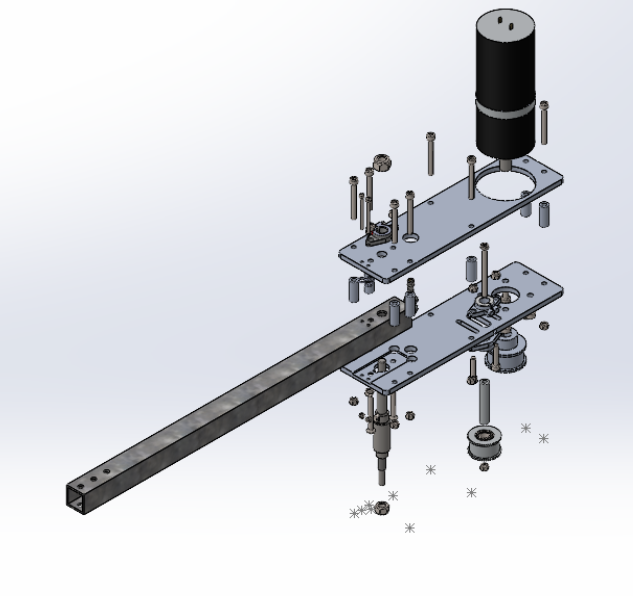
\includegraphics[width=0.8\textwidth]{images/Arm_explode.png}
    \caption{รูป Exploded View ของส่วนแขนกลและข้อต่อในมุม Isometric}
    \label{fig:arm_exploded_iso}
\end{figure}

\textbf{4. ส่วนชุดเอ็นโค้ดเดอร์ (Encoder Sub-assembly)}
\begin{figure}[H]
    \centering
    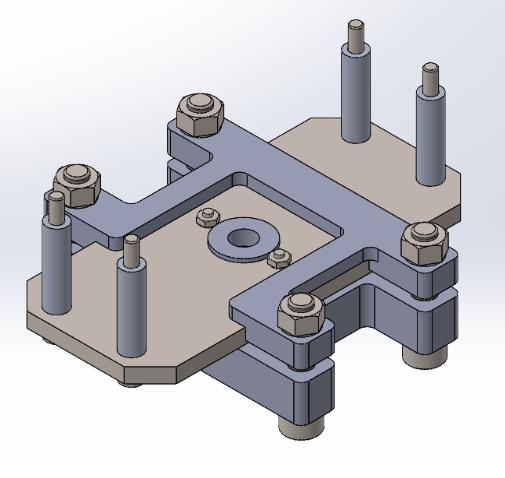
\includegraphics[width=0.7\textwidth]{images/encoder_subassem.png}
    \caption{ภาพรวมของ ส่วน Encode ในมุม Isometric}
    \label{fig:encoder_iso}
\end{figure}
\begin{figure}[H]
    \centering
    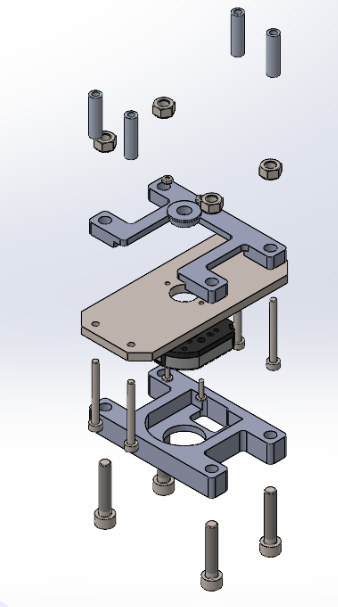
\includegraphics[width=0.8\textwidth]{images/encoder_explode.png}
    \caption{รูป Exploded View ของ ส่วน Encode มุม Side view และ Isometric}
    \label{fig:encoder_exploded}
\end{figure}

\textbf{5. Part จัดระเบียบสายไฟ}
\begin{figure}[H]
    \centering
    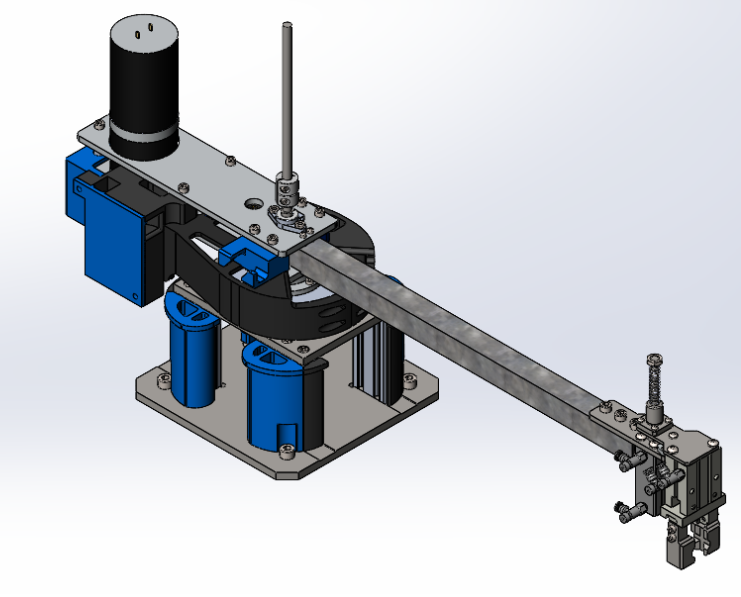
\includegraphics[width=0.7\textwidth]{images/full_assem.png}
    \caption{รูปหุ่นที่มี part จัดระเบียบสายไฟ ในมุม Isometric}
    \label{fig:cable_mgt_iso}
\end{figure}
\begin{figure}[H]
    \centering
    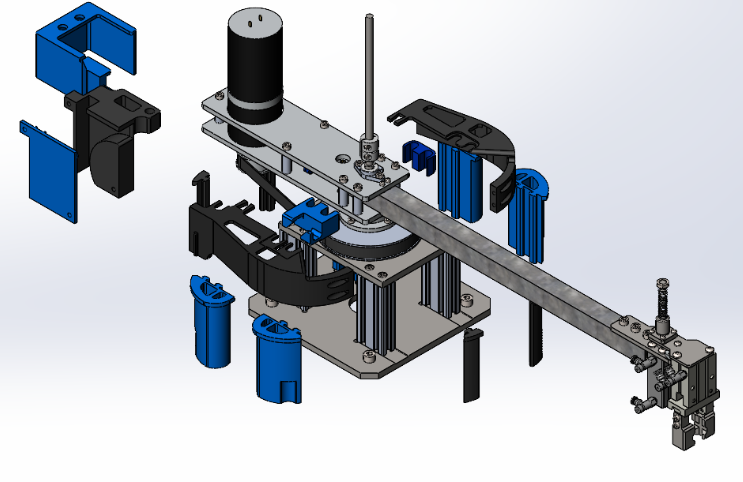
\includegraphics[width=0.8\textwidth]{images/full_explode.png}
    \caption{รูป Exploded View ของหุ่นที่มี part จัดระเบียบสายไฟ ในมุม Isometric}
    \label{fig:cable_mgt_exploded}
\end{figure}

% ------------------------------------------------------------
\subsection{Drawing แต่ละชิ้นส่วน}
\label{subsec:part_drawings}
% ------------------------------------------------------------

\begin{figure}[H]
  \centering
  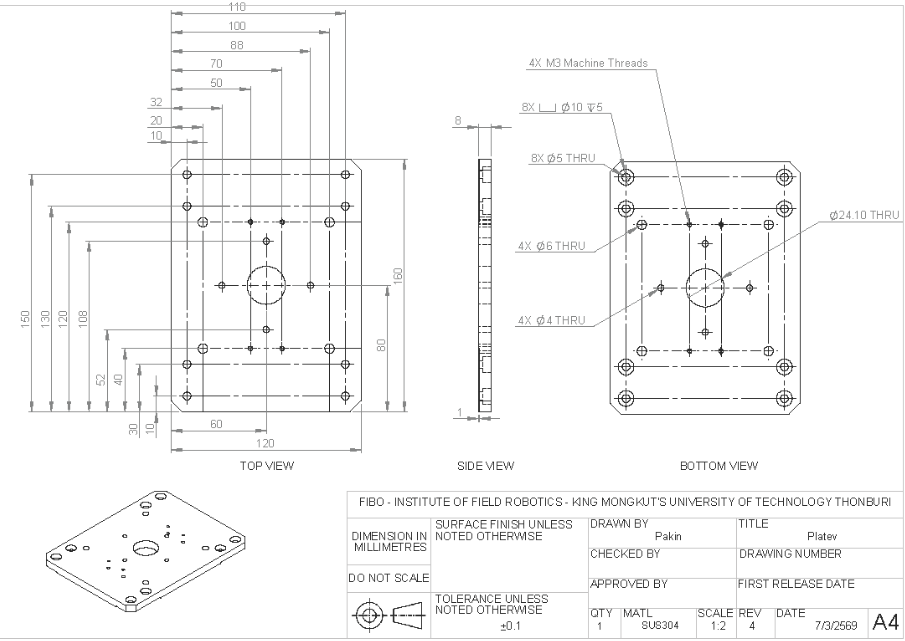
\includegraphics[width=0.95\textwidth]{images/Drawing_PlateV.png}
  \caption{Engineering Drawing: Base Plate}
  \label{fig:app_draw_base}
\end{figure}

\begin{figure}[H]
  \centering
  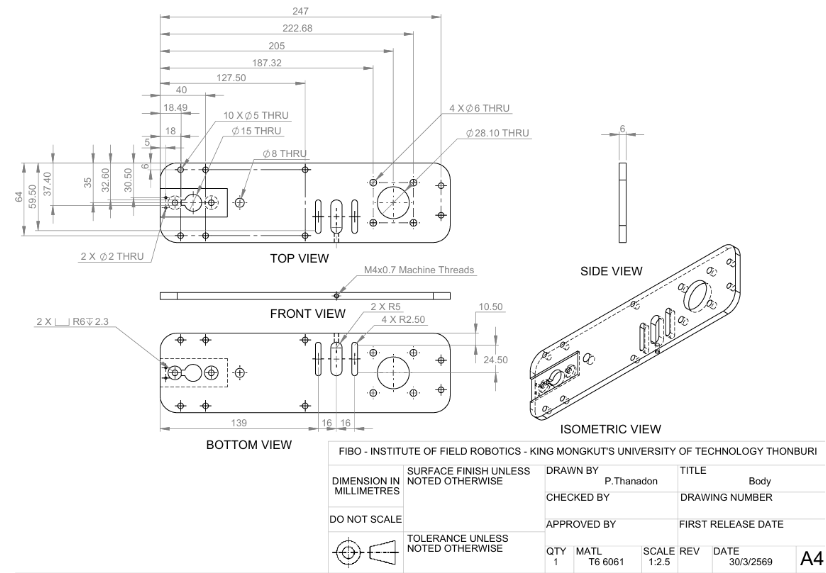
\includegraphics[width=0.95\textwidth]{images/Drawing_Body.png}
  \caption{Engineering Drawing: Body Plate}
  \label{fig:app_draw_body}
\end{figure}

\begin{figure}[H]
  \centering
  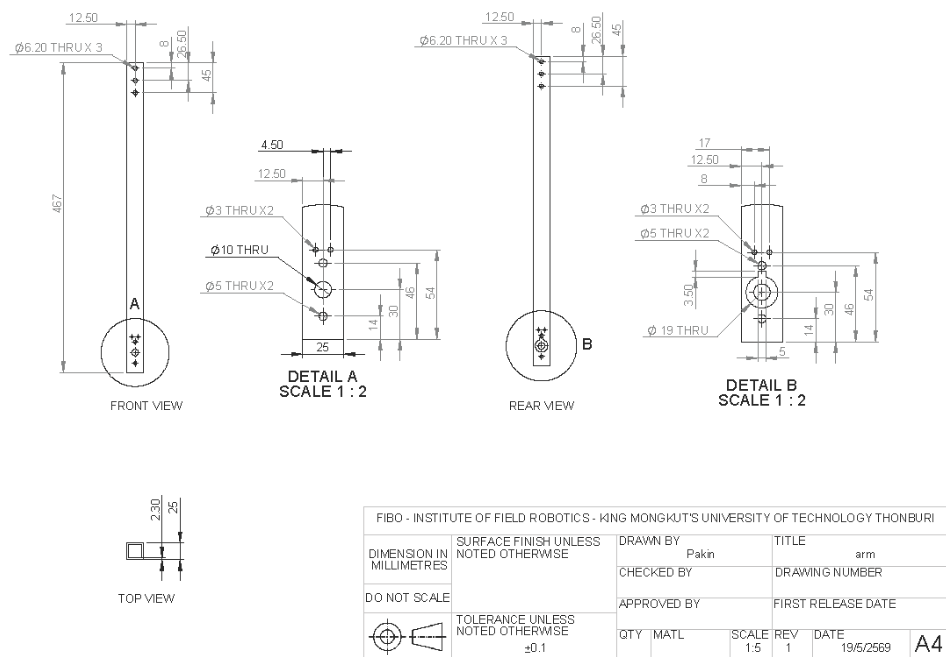
\includegraphics[width=0.95\textwidth]{images/Drawing_Arm.png}
  \caption{Engineering Drawing: Rotating Arm}
  \label{fig:app_draw_arm}
\end{figure}

\begin{figure}[H]
  \centering
  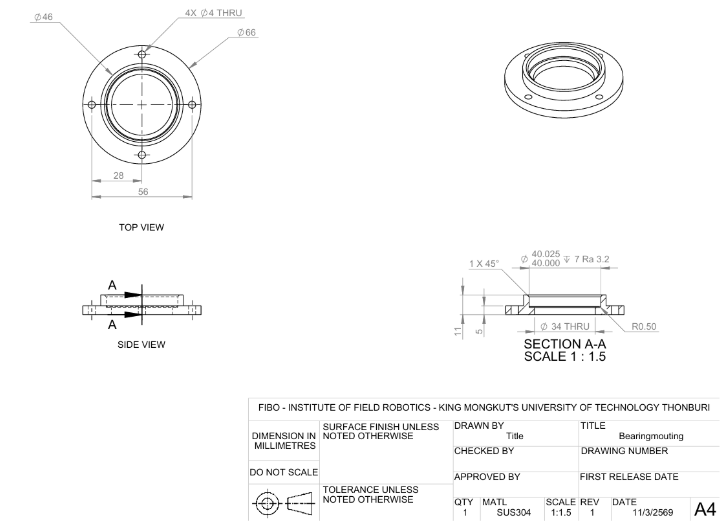
\includegraphics[width=0.95\textwidth]{images/Drawing_Bearingmounting.png}
  \caption{Engineering Drawing: Bearing Mounting}
  \label{fig:app_draw_azimuth}
\end{figure}

\begin{figure}[H]
  \centering
  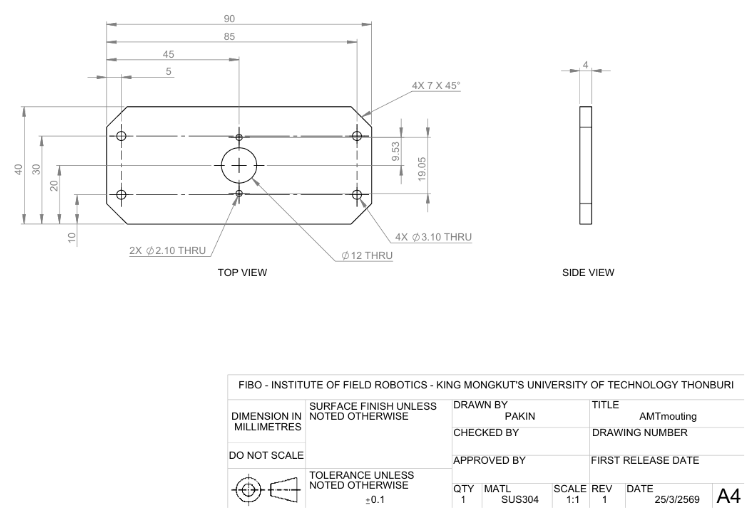
\includegraphics[width=0.95\textwidth]{images/Drawing_MoutingEncoder.png}
  \caption{Engineering Drawing: Encoder Housing}
  \label{fig:app_draw_encoder}
\end{figure}

\begin{figure}[H]
  \centering
  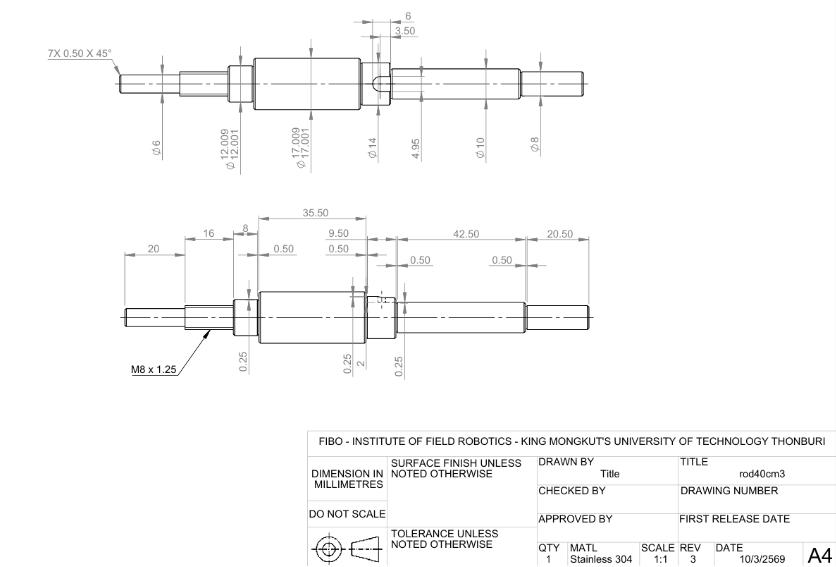
\includegraphics[width=0.95\textwidth]{images/Drawing_Rod40.png}
  \caption{Engineering Drawing: Rod40}
  \label{fig:app_draw_ee}
\end{figure}

\begin{figure}[H]
  \centering
  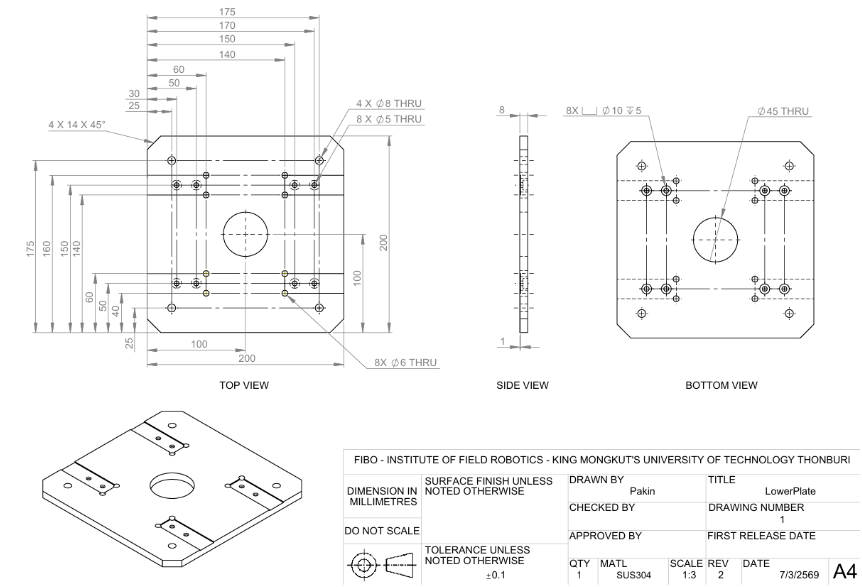
\includegraphics[width=0.95\textwidth]{images/Drawing_Lowerplate.png}
  \caption{Engineering Drawing: Lower plate}
  \label{fig:app_draw_actuator}
\end{figure}

\begin{figure}[H]
  \centering
  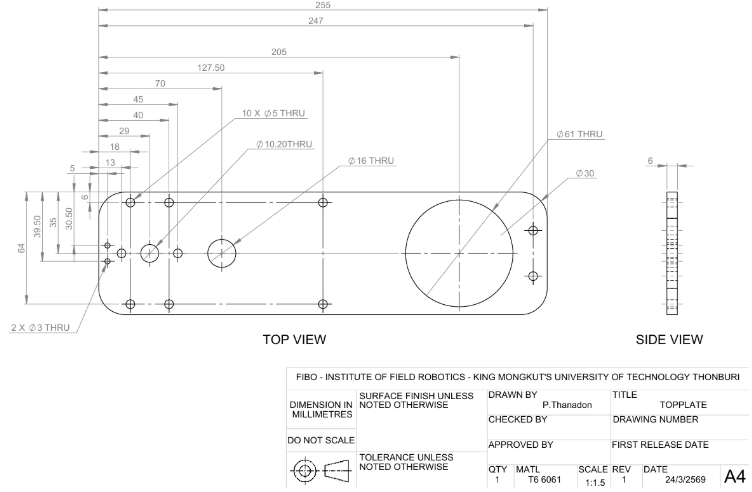
\includegraphics[width=0.95\textwidth]{images/Drawing_Topplate.png}
  \caption{Engineering Drawing: Top plate}
  \label{fig:app_draw_actuator}
\end{figure}


%--------------------------------------------------------------------

\section{รายละเอียดการคำนวณเชิงกล}
\label{sec:mechanical_calculation_details}
% การคำนวณฉบับเต็ม Shaft, Belt, Bearing, Deflection
% อ้างอิงไฟล์ PDF ที่มีอยู่แล้วใน Project
\subsubsection{การคำนวณแรงบิดและการเลือกมอเตอร์}
\label{subsubsec:motor_torque_calculation}

การคำนวณนี้มีวัตถุประสงค์เพื่อพิสูจน์ว่าชุดมอเตอร์ที่เลือก (RS-775246000 + Planetary Gearbox + Belt) มีแรงบิดเพียงพอที่จะขับแขนกลให้เป็นไปตาม Requirements P3 และ P4 ภายใต้โหลดสูงสุด

ความเฉื่อยรวมของระบบ ($J_{total}$) ได้จากการวิเคราะห์ SolidWorks Model ซึ่งครอบคลุมมวลแขนกล, End Effector, และโหลดสูงสุด 2 kg:

% \begin{figure}[H]
%     \centering
%     \includegraphics[width=0.7\textwidth]{images/solidworks_inertia.png}
%     \caption{ภาพแสดงการวิเคราะห์ความเฉื่อยรวมของระบบจากโปรแกรม SolidWorks}
%     \label{fig:solidworks_inertia}
% \end{figure}

\begin{equation}
    J_{total} = 0.5764 \text{ kg}\cdot\text{m}^2 \quad \text{(จาก SolidWorks)}
    \label{eq:inertia_total}
\end{equation}

แรงบิดที่ต้องการ ($T_{req}$) คำนวณจากกฎของนิวตันสำหรับระบบหมุน:
\begin{equation}
    T_{req} = J_{total} \times \alpha_{min} = 0.5764 \times 2.0 = 1.153 \text{ Nm}
    \label{eq:torque_required}
\end{equation}

รวม Safety Factor = 2 เพื่อรองรับแรงเสียดทานและความไม่แน่นอนในระบบ:
\begin{equation}
    T_{final} = T_{req} \times SF = 1.153 \times 2.0 = 2.306 \text{ Nm}
    \label{eq:torque_final}
\end{equation}

แรงบิดที่ระบบสามารถส่งออกได้จริงที่เพลาแขนกล คำนวณจากห่วงโซ่การส่งกำลังทั้งหมด:
\begin{equation}
    T_{arm} = T_{motor} \times i_{gear} \times \eta_{gear} \times i_{belt} \times \eta_{belt}
    \label{eq:torque_arm_formula}
\end{equation}
\begin{equation}
    T_{arm} = 0.0955 \times 24 \times 0.85 \times 3 \times 0.95 = 5.3977 \text{ Nm}
    \label{eq:torque_arm_result}
\end{equation}

Safety Factor ที่ได้จริง:
\begin{equation}
    SF_{actual} = \frac{T_{arm}}{T_{req}} = \frac{5.3977}{1.153} = 4.682
    \label{eq:safety_factor_actual}
\end{equation}

\begin{table}[H]
    \centering
    \caption{ตารางสรุปผลการคำนวณการขับเคลื่อนและ Safety Factor}
    \label{tab:motor_calc_summary}
    \begin{tabular}{|p{0.38\textwidth}|p{0.25\textwidth}|p{0.27\textwidth}|}
        \hline
        \textbf{พารามิเตอร์} & \textbf{ค่า} & \textbf{หมายเหตุ} \\
        \hline
        ความเฉื่อยรวม (จาก SolidWorks) & $J_{total} = 0.5764 \text{ kg}\cdot\text{m}^2$ & ครอบคลุมแขนกล, End Effector, และโหลด \\
        \hline
        ความเร่งเชิงมุมที่คำนวณได้ & $\alpha_{max} = 9.3641 \text{ rad/s}^2$ & มากกว่า Requirement P4 ($\geq 2.0 \text{ rad/s}^2$) \\
        \hline
        ความเร็วเชิงมุมที่คำนวณได้ & $\omega_{arm} = 8.9760 \text{ rad/s}$ & มากกว่า Requirement P3 ($\geq 2.9 \text{ rad/s}$) \\
        \hline
        แรงบิดที่มอเตอร์ต้นกำลัง & $T_{motor} = 0.0955 \text{ Nm}$ & จาก Datasheet มอเตอร์ \\
        \hline
        อัตราทด Planetary Gearbox & $i_{gear} = 24:1$ & ภายในชุด Gearmotor \\
        \hline
        ประสิทธิภาพ Gearmotor & $\eta_{gear} = 0.85$ & - \\
        \hline
        แรงบิดหลัง Gearbox & $T_{gear} = 1.9481 \text{ Nm}$ & $T_{motor} \times i_{gear} \times \eta_{gear}$ \\
        \hline
        อัตราทดสายพาน (Driven 72T : Driver 24T) & $i_{belt} = 3:1$ & - \\
        \hline
        ประสิทธิภาพสายพาน & $\eta_{belt} = 0.95$ & - \\
        \hline
        แรงบิดรวมที่เพลาแขนกล & $T_{arm} = 5.3977 \text{ Nm}$ & $T_{gear} \times i_{belt} \times \eta_{belt}$ \\
        \hline
        Safety Factor ที่ได้ & $SF = 4.682$ & $\geq 2.0$ (ตาม Requirement) \\
        \hline
    \end{tabular}
\end{table}

\textbf{สรุปผลการตรวจสอบ:} 
จากผลการคำนวณพบว่า $SF_{actual} (4.682) > SF_{req} (2.0)$ และ $T_{arm} (5.3977 \text{ Nm}) > T_{final} (2.306 \text{ Nm})$ ดังนั้นระบบจึงผ่านข้อกำหนดด้านแรงบิดและ Safety Factor อย่างสมบูรณ์


\section{รายละเอียดการคำนวณ Motion Profile}
\label{sec:motion_profile_calculation_details}
% การคำนวณ S-Curve ฉบับเต็ม ทุกช่วง (Acceleration, Constant, Deceleration)

\section{Schematic ไฟฟ้าฉบับเต็ม}
\label{sec:full_electrical_schematic}
% Schematic ขนาดเต็มอ่านได้ง่าย

\begin{figure}[H]
  \centering
%   \includegraphics[width=0.95\textwidth]{images/schematic_full.png}
  % [ใส่ภาพ Schematic ขนาดเต็ม]
  \caption{Electrical Schematic ฉบับเต็ม}
  \label{fig:schematic_full}
\end{figure}

\section{Code Snippet หลักของ STM32 Firmware}
\label{sec:firmware_code_snippets}
% Code สำคัญ เช่น PID Loop, Encoder Read, S-Curve Generator
% ใช้ lstlisting environment

\begin{lstlisting}[language=C, caption={ตัวอย่าง PID Control Loop บน STM32}]
/* [ใส่ Code จริงของ PID Loop] */
\end{lstlisting}

\section{ผลการ Simulation Simscape ฉบับเต็ม}
\label{sec:simscape_simulation_results}
% Plot และผลลัพธ์จาก Simscape ทุก Scenario

\begin{figure}[H]
  \centering
%   \includegraphics[width=0.85\textwidth]{images/simscape_full_result.png}
  % [ใส่ Plot ทั้งหมดจาก Simscape: Position, Velocity, Control Effort]
  \caption{ผล Simulation Simscape ฉบับเต็ม}
  \label{fig:simscape_full}
\end{figure}

\section{Log การทดสอบ Unit Test}
\label{sec:unit_test_logs}
% Serial Log, Oscilloscope Screenshot จากการทดสอบต่างๆ

\begin{figure}[H]
  \centering
%   \includegraphics[width=0.80\textwidth]{images/serial_log_encoder.png}
  % [ใส่ภาพ Serial Monitor Log แสดงค่า Encoder ขณะทดสอบ]
  \caption{Serial Log ขณะทดสอบการอ่านค่า Encoder}
  \label{fig:serial_log}
\end{figure}